\documentclass{sig-alternate}

\usepackage{graphicx}
\usepackage{subfig}
\usepackage{url}
\usepackage{verbatim}
\usepackage{xspace}

\usepackage{watermark}

\DeclareCaptionType{copyrightbox}
%\usepackage{etoolbox}
%\makeatletter
%\patchcmd{\maketitle}{\@copyrightspace}{}{}{}
%\makeatother
%\sloppy

\newcommand{\eg}{e.g.\xspace}
\newcommand{\ie}{i.e.\xspace}
\newcommand{\etc}{etc.\xspace}
\newcommand{\etal}{et al.\xspace}
\newcommand{\vect}[1]{\ensuremath{\overrightarrow{#1}}}
\newcommand{\tm}[1]{\emph{#1}}

\newcommand{\namesep}{\hspace{1cm}}
\toappear{}
%\renewcommand{\baselinestretch}{0.937}

\special{! /pdfmark where
  {pop} {userdict /pdfmark /cleartomark load put} ifelse [
    /Author ()
    /Title (NormSTAD Flight Analysis: Visualizing Air Traffic Patterns over the United States)
    /Keywords ()
    /DOCINFO pdfmark}


\title{NormSTAD Flight Analysis: Visualizing Air Traffic Patterns over the United States
}%\vspace{-20pt}}


\numberofauthors{1}
\author{
\alignauthor
\begin{tabular}{c@{\namesep}c@{\namesep}c}
 Samet Ayhan & Brendan C. Fruin & Fan Yang
\end{tabular}\\
\affaddr{Department of Computer Science, University of Maryland}\\
\affaddr{College Park, MD  20742 USA}
\email{\{sayhan, brendan, fyang\}@cs.umd.edu}
}

\newcommand{\refname}{Bibliography}

\begin{document}

\maketitle

\begin{abstract}

In this paper, we describe the NormSTAD Flight Analysis Tool, a novel interactive 
visualization application
of air traffic patterns using Aircraft
Situations Display to Industry (ASDI) data. A web-based visualization
is demonstrated which allows users to analyze flight data and make 
discoveries pertaining to their 4D trajectories which include 
their time, distance, altitude, and speed. Unique patterns discovered
in this application could result in less fuel consumption and more efficient
management of departure and arrivals by air traffic controllers.

The application consumes ASDI data then normalizes flight attributes
including distance, speed, altitude, and time along the flight path. This 
information is then displayed on a line chart which can be customized
through filtering, coloring and selection. Attributes pertaining to 
selected flights can be viewed in a details on demand fashion. The result
is a both intuitive and visually appealling visualization with the goals
of revealing flight paths, spotting trends and revealing outliers.

\end{abstract}

\category{H.3.3}{Information Storage and Retrieval}{Information Search and Retrieval}[Information filtering]
\category{\\H.3.5}{Information Storage and Retrieval}{Online Information Services}[Web-based services]
\category{\\H.5.2}{Information Interfaces and Presentation}{User Interfaces}

\vspace{-2mm}
\terms{Design, Human Factors, Performance}



\section{Introduction}
\label{sec-introduction}

The National Airspace System (NAS) is a complex non-deterministic system that
is impacted continually by both major and minor variables including aircraft
delays and human decisions that largely cannot be accurately forecasted.
The system has developed to offer feedback and response at all levels from
gate agents to the Command Center with the intent of restoring the desired
efficient state. The result is a self-ordering system that is broadly
similar, but has different daily operations. An important point to note is that
a seemingly insignificant event such as
a delay in obtaining a wheel chair can have large impacts in delays
as \emph{slots} are missed and reassigned. At every stage decisions are being
made to recover the system and keep it as close to optimal given its current
state. However, there is currently no method of quantifying the effects of 
a decision or comparing them to an alternate decision. NAS operations
are recorded concurrently across different systems in different formats.
If this information was collated and catalogued, it would be possible
to analyze the NAS operations to identify inefficiencies, disruptive events 
and poor decisions along with the resulting impacts on airspace users.

In 1992 the Federal Aviation Administration (FAA), started a program to provide
real-time flight plan and track information for the NAS to airlines and other
oganizations. The feed known as Aircraft Situation Display to Industry (ASDI) is a 
product of the Enhanced Traffic Management System (ETMS). It originates from
the Traffic Flow Management (TFM) Production Center located at the William
J. Hughes Technical Center in Atlantic City, New Jersey. Figure~\ref{table1} shows the 
number of ASDI messages for a single random day while Figure~\ref{table2} shows the number
of supporting records for the main message set. As can be by Figure~\ref{two-tables},
tens of millions of ASDI messages are recorded each day.


A novel visualization system is needed to aggregate this data in order for 
users to detect anomalies and discover unique patterns. To be able to compare 
flights of varying distance or time, the data values are normalized to 
create a standardized display of time series allowing direct comparison between
flights. 

\newcommand{\incfig}[2]{\includegraphics[#2]{figs/#1}\label{#1}}

\begin{figure}
\centering
\subfloat[]{\incfig{table1}{width=1\columnwidth}}\hfill
\subfloat[]{\incfig{table2}{width=1\columnwidth}}
\caption{
(a) Table displaying the number of ASDI messages in a given day
(b) Table displaying the number of supporting records for main ASDI message set
% \subref{table2} Caption for Figure 1b -- SAMET
}
\label{two-tables}
\end{figure}

The rest of this paper is organized as follows. Section~\ref{sec-related-work}
discusses related
work. Section~\ref{sec-asdi} explains the ASDI data and its attributes. 
Section~\ref{sec-architecture} describes
the overall architecture and the interface is described in Section~\ref{sec-interface}.
Section~\ref{sec-expert-review}
provides the expert reviews
and feedbacks of the implementation. Section~\ref{sec-future-work}
discusses future work, while our conclusions
are outlined in Section~\ref{sec-conclusion}.

\section{Related Work}
\label{sec-related-work}

There has been a great amount of research in flight data pertaining to algorithms
for optimal trajectories, anomaly detection and conflict 
resolution~\cite{Basu09, Cao06, Chu10, Liu08, Rama06, Wang04}.
Liu et al.~\cite{Liu08} studied departure and arrival delays and how these delays
can propagate to future flight delays and cancellations. Our system instead focuses
on in-air flight data to help study why these delays may be happening with 
respect to time of day, flight number, airline or flight trajectory. 
Chu et al.~\cite{Chu10} had a similar approach to NormSTAD in that they
attempted to detect anomalies in aircraft cruise data by using time, location, altitude 
and speed. They also normalized their data as was done in the NormSTAD tool. However,
the NormSTAD tool utilizes historical data while their system studied the results
of a simulation. While the study of such algorithms for detection of anomalies and conflict
resolution is vitally important to the field of aviation, the goal of the NormSTAD Flight Analysis 
Tool is to allow easy and timely analysis of large amounts of flight data without the need
for such algorithms.

Landry~\cite{Landry11} and Khoury et al.~\cite{Khoury06} stress the importance
of informative visualizations for the study of air traffic control systems.
Landry reviewed and analyzed the current air traffic control system which 
has evolved around the air traffic controller and pilots while not 
updating to the increasing air traffic. Landry states that the 
current visualizations may not concisely display the operator with the 
necessary information. Khoury et al. focus their attention on 
construction of a 3D model of only airport operations. Their analysis of delays
is limited in that they do not include flight sensory data in their analysis.

Many other researchers have created flight data 
visualizations~\cite{Conv2011, Hurter10, Klein06, Palmer08, Pestana05}.
Hurter et al.~\cite{Hurter10} designed a metro style visualization
for flight paths in the Air Traffic Control context in
order to avoid severe overlaps of the lines
along with a complete method to produce an efficient layout.
This visualization is clear and visually appealing, but fails 
to inform the user of differences in flight paths since it 
does not use the actual latitude and longitude coordinates
of the flight. The AIRNET platform by Pestana et al.~\cite{Pestana05}
provides a 3D model for surveillance, control, guidance and decision
support services by airport operators. The NormSTAD tool avoids
3D visualization to reduce complexity by allowing the axes to be changed  
by the user.

After reviewing the current state-of-the-art of flight visualizations,
we decided to follow Wehrend's ideas~\cite{Weh90}. Wehrend believes
that visualizations should break problems into smaller problems
and find applicable techniques for each of these smaller problems.
The visualization is then a unified representation of the smaller
problems in order to solve larger problems. It is with this belief
that the NormSTAD Flight Analysis Tool was based and designed
using four connected view panels for information display and interaction. 
The Filters panel allows for data filtering which is separated from 
our data visualization and selection Line Chart. Details on demand
are displayed in two separate panels, the Map and Details on Demand panel. 
Using this application,
airline operators will be able to better determine flight plans,
discover holding and slow-down patterns caused by disruptive events, consume
less fuel and save time, money and the environment in the process. 



\section{ASDI Data}
\label{sec-asdi}

In this section, we introduce ASDI data and its
attributes. In addition, we describe the data normalization
process that NormSTAD uses.

The ASDI subsystem of the Traffic Flow
Management System (TFMS)~\cite{TFMS} allows near
real-time air traffic data to be disseminated to
members of the aviation industry. The data stream
is made available through the U.S. Department
of Transportation's Volpe Transportation Center.
The data stream consists of data elements which
show the position and flight plans of all aircrafts
in the United States. Attributes include the location, altitude,
airspeed, destination, estimated time of arrival and
tail number or designated identifier of air carrier
and general aviation aircraft operating on IFR flight
plans within the United States airspace.

Due to the limitations in the web tools employed by NormSTAD, only a
subset of the historical ASDI data was used. The data
set included Delta Airlines' and Delta Connection, Atlantic
Southeast Airlines' flights departing from Seattle
Tacoma Airport (KSEA) for the duration of July
and August 2012.

Flights pertaining to Delta Airlines consisted
of the following flight numbers:
\begin{itemize}
\item[$\cdot$] DAL842, departing from Seattle Tacoma
and arriving at New York JFK
\item[$\cdot$]  DAL1043, departing from Seattle Tacoma
and arriving at New York JFK Airport
\item[$\cdot$]  DAL2410, departing from Seattle Tacoma
and arriving at Detroit Metropolitan
Wayne  County Airport
\end{itemize}

Flights pertaining to Delta Connection,
Atlantic Southeast Airlines consisted of the
following flight numbers:
\begin{itemize}
\item[$\cdot$] ASA24, departing from Seattle Tacoma
and arriving at Boston Logan International
Airport
\item[$\cdot$]  ASA678, departing from Seattle Tacoma
and arriving at Denver International
Airport
\end{itemize}

The dataset was generated by merging a subset of
various message types including:
\begin{itemize}
\item[$\cdot$] Departure Information
\item[$\cdot$] Track Information
\item[$\cdot$] Flight Management Information
\end{itemize}

The process yielded the following fields:
\begin{itemize}
\item[$\cdot$] Source Date
\item[$\cdot$] Source Time
\item[$\cdot$] Aircraft Id
\item[$\cdot$] Speed
\item[$\cdot$] Altitude
\item[$\cdot$] Latitude
\item[$\cdot$] Longitude
\end{itemize}


In addition, certain values were normalized
so that various flights or time series of different
flights could be overlaid on the same line chart.
Normalized values for interactive visualization
included:
\begin{itemize}
\item[$\cdot$] Altitude
\item[$\cdot$] Speed
\item[$\cdot$] Distance
\item[$\cdot$] Planned Flight Time 
\item[$\cdot$] Actual Flight Time
\end{itemize}

Normalized values range between 0 and 1
where 0 denotes the minimum possible for a given value (i.e. the departure airport
in the case of distance) and 1 denotes the maximum possible 
for a given value (i.e. the arrival airport in the case of distance) 
for all values with the exception that Actual Flight Time may
exceed 1 or be below 1 due to the fact that it does not correspond exactly 
to the Planned Flight Time.


\section{Implementation}
\label{sec-architecture}

The NormSTAD Flight Analysis Tool is a web-based implementation which is primarily built
using the D3 JavaScript library. D3, which stands for Data-Driven Documents, is a 
library that allows users to bind arbitrary data with a Document Object Model (DOM)
and achieve data-driven transformations~\cite{D3}. NormSTAD utilizes a predefined API of D3
to import our data from a local file
 and store the normalized values of time, distance, speed and altitude
for each flight. Flight information including flight number, airline and date are also imported
using D3. After the data is finished being imported, the filters are dynamically created.

All filters in the Filters section
 are created using HTML syntax and JavaScript apart from the input text bar
to search for a specific flight which is created using jQuery~\cite{jQuery}.
Filters to select airlines and flights are bound to the imported data using D3 so that
they can update the visualization accordingly. Filters to select the date of flights
are created using the DHTMLX~\cite{DHTMLX} JavaScript library.

Drop down menus for choosing the line chart type and color and the checkbox for map display
are implemented in JavaScript with events handled in D3 to link filters with the line chart.
The NVD3~\cite{NVD3} JavaScript library is used for the line chart, horizontal axis 
selection and the legend. The Google Maps JavaScript API~\cite{API} provides our flight path map,
airport markers and flight path drawing. The Details on Demand panel is a dynamic
HTML table which changes as a result of selection in the line chart.



\section{User Interface}
\label{sec-interface}

The NormSTAD Flight Analysis user interface initially shows four panels of display as seen in 
Figure~\ref{speed} labeled Filters, Line Chart, Map and Details on Demand. Each panel allows for 
direct interaction or display of the data and can be minimized to
give more room to the other panels by selecting 
the arrow in the upper right corner of the specific panel. In the following sub sections, we 
will introduce each panel to give readers a better sense of the functionality of the 
NormSTAD Flight Analysis Tool.

\begin{figure}
\centering
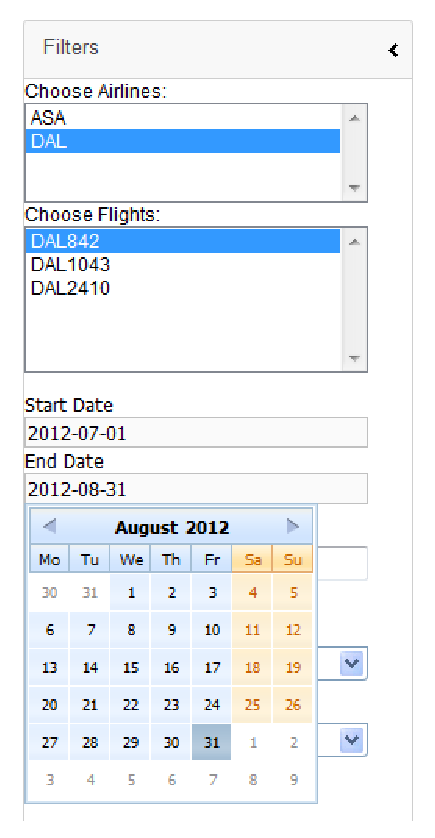
\includegraphics[height=3.5in]{figs/calendar.eps}
\caption{
	Filters of NormSTAD Flight Analysis Tool's interface where date selection text box
displays a calendar allowing users to select a date.
}
\label{calendar}
\end{figure}


\begin{figure*}
\centering
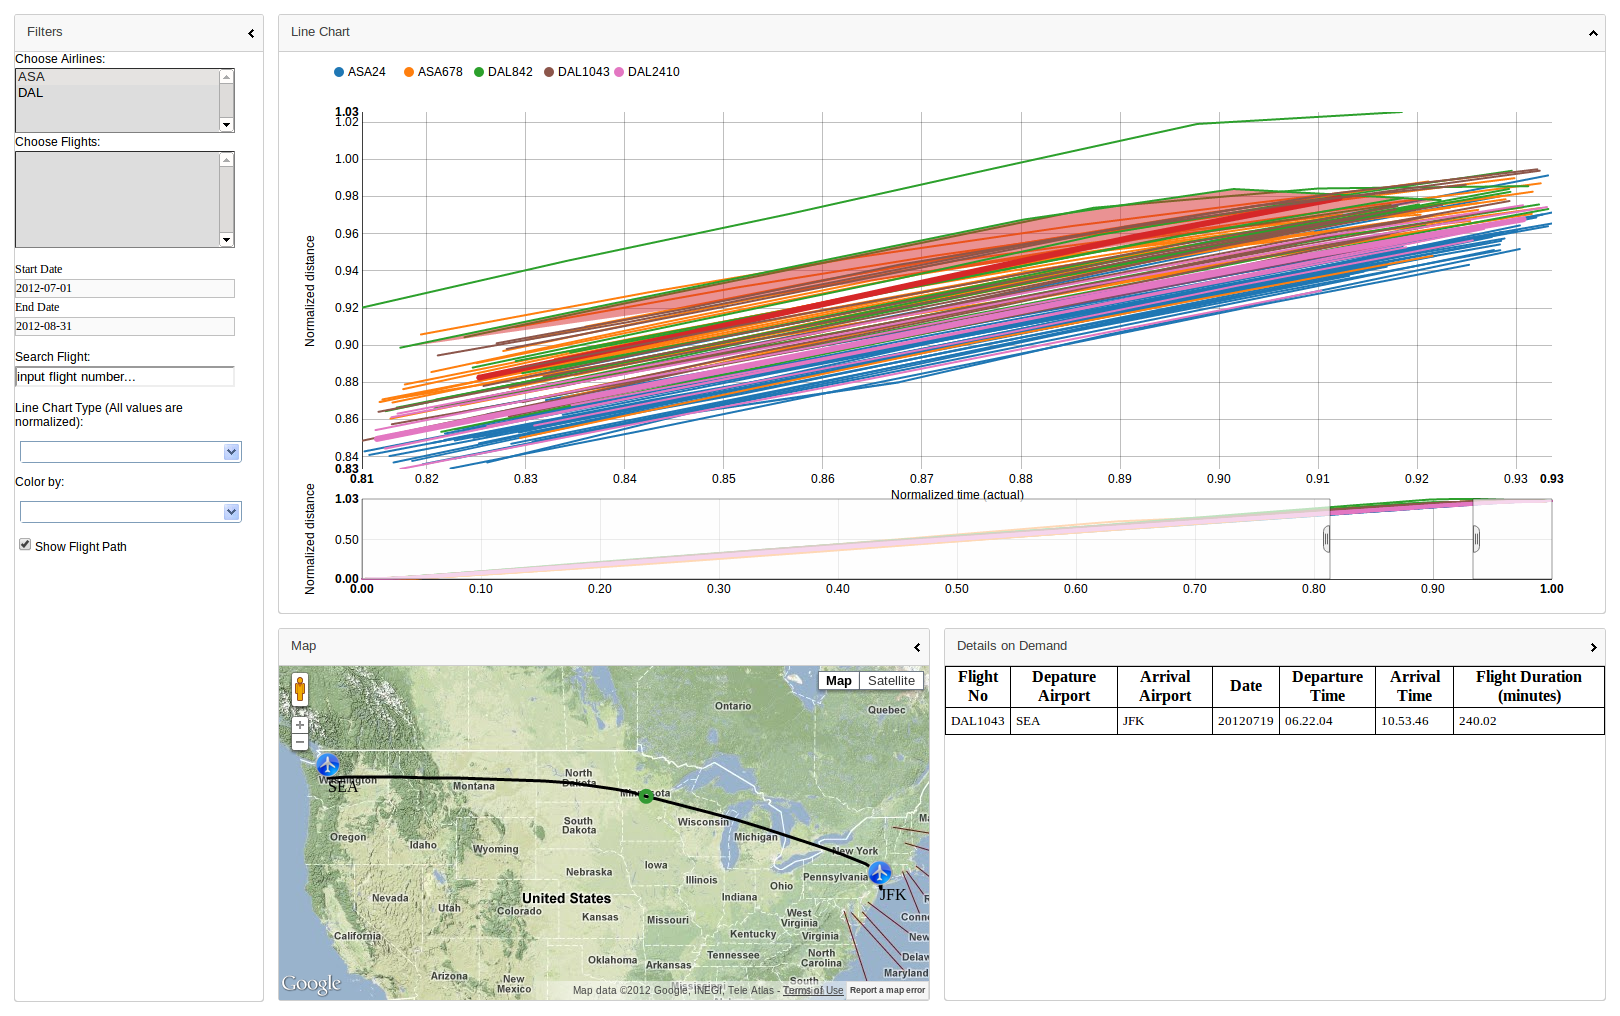
\includegraphics[width=\textwidth]{figs/overview.eps}
\caption{
NormSTAD Flight Analysis Tool's interface showing Normalized Actual Flight Time
for the range from 0.81 to 0.93 with 
respect to Normalized Distance. One flight is selected (red line) with its 
corresponding path shown on the map and details in Details on Demand.
}
\label{overview}
\end{figure*}

\begin{figure*}
\centering
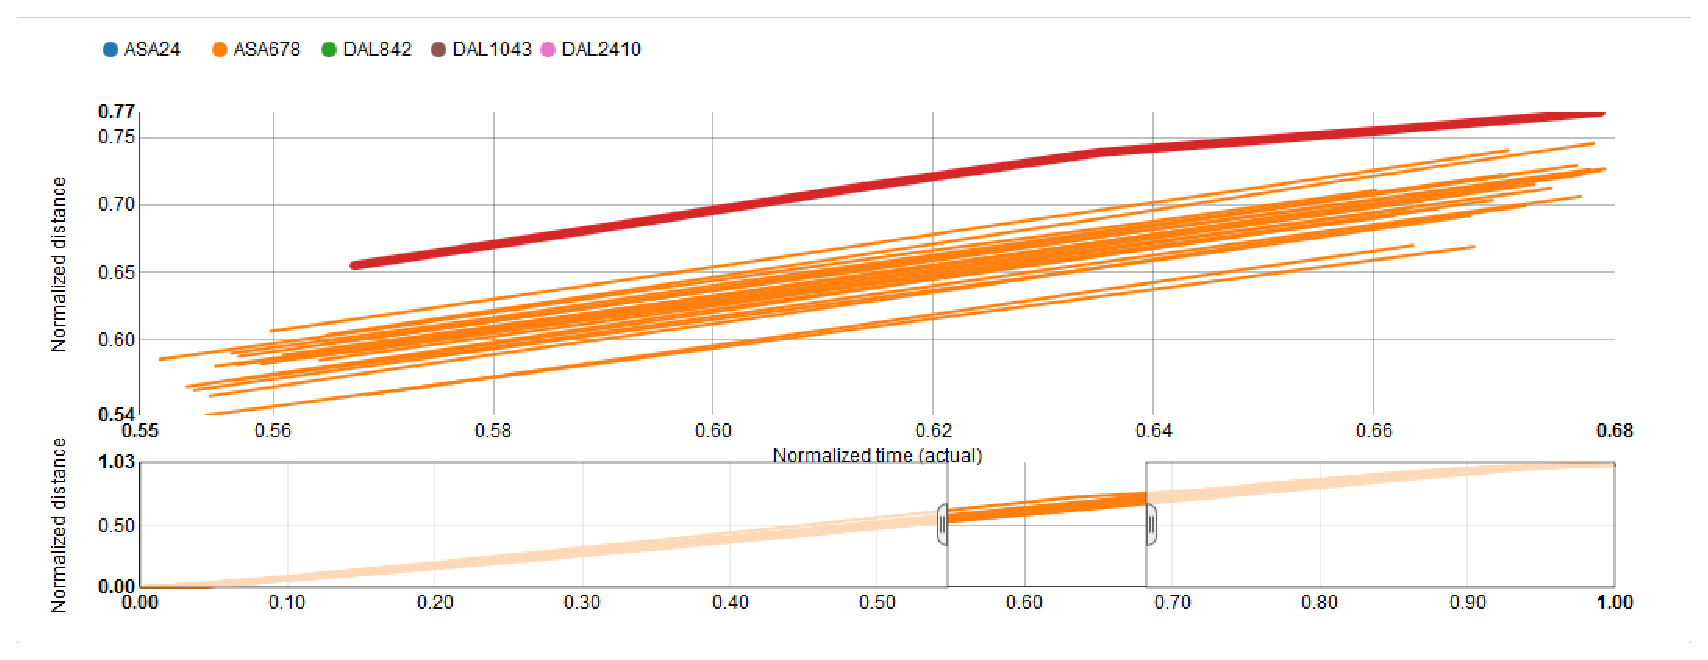
\includegraphics[width=\textwidth]{figs/outlier.eps}
\caption{}
\label{outlier}
\end{figure*}


\begin{figure*}
\centering
\subfloat[]{\incfig{speed}{width=\textwidth}}\hfill
\subfloat[]{\incfig{linechart3}{width=\textwidth}}
\caption{
(a) Filtering to display only the Normalized Speed vs. the Normalized Actual Flight Time for the range from 0.4 to 0.6 along the horizontal axis for flights ASA24 and DAL842. Flights are colored by airline.
(b) Displaying Normalized Altitude vs. the Normalized Actual Flight Time colored by flight number.}
\label{lines}
\end{figure*}
 
\subsection{Filters}
\label{subsec-filters}

On the left-side of the tool, there is a Filters panel which allows the user
to limited the results taht they see on the Line Chart. The first section,
``Choose Airlines", is for selection of airlines to display in the 
Line Chart which is set to all airlines by default after the data is loaded.
Upon selection of an airline, the Line Chat is updated accordingly and 
the ``Choose Flights" section is populated with all flights
for the selected airline(s). Note that a user can select
multiple adjacent rows for both the Choose Airlines and the Choose Flights
sections by holding the Shift key and selecting rows or multiple rows
by holding the Control key (Apple key on Apple computers) and selecting rows as 
seen in Figure~\ref{speed}.
Selection of row(s) in the Choose Flights section allows for updating 
of the Line Chart by the flight number. The flights can be further filtered 
by limiting the flight date using the ``Start Date" and ``End Date" drop-down 
calendar menus. The Start Date refers to the departure date of a flight
while the End Date refers to the arrival date of a flight. As shown in
Figure~\ref{calendar}, a calendar is popluated after a user clicks the text box.
Users can then easily select two dates to filter the date range of flights 
to show in the Line Chart. Below the date selector, there is a search bar which 
allows specific flights to be shown.


Apart from filters to control the flights shown in the Line Chart, NormSTAD also allows changing
of the attributes displayed and the color of the lines in the Line Chart. The ``Line Chart Type"
value changes the axes and updates the normalized data displayed. By default, this value
is set to ``Distance vs. Actual Flight Time", but it can be changed to ``Distance
vs. Planned Flight Time", ``Altitude vs. Actual Flight Time", or ``Speed vs. Actual Flight Time". 
The line can be colored by their airline or by their flight number using the ``Color by" drop-down
menu. After changining the color, the legend above the Line Chart updates with the new 
color scheme. In Figure~\ref{speed}, we show ``Speed vs. Actual Flight Time" colored by
airline and in
Figure~\ref{linechart3} we show
``Altitude vs. Actual Flight Time" Line Chart colored by flight number. 

\subsection{Line Chart}
\label{subsec-linechart}
The top center of the browser is occupied by the Line Chart which provides a graphical
visualization for different attributes. When the application is first opened,
the Line Chart panel of NormSTAD presents two graphs with all flights displayed for the loaded
dataset. In implementing the Line Chart, we encountered a noticeable issue in that lines are often
close together and hard to distinguish. It is almost impossible for users to find any useful insights
given such crowded lines. To combat this issue, we introduce an additional graph below the main
Line Chart allowing for selection of a range of the horizontal axis. By selecting a range along 
the horizontal axis, the coordinate system of the top graph is redrawn to have only values contained within
the selected subset creating a zoom-in effect. This range can be expanded or contracted and even moved
by clicking, holding, and dragging the range window. A mouse hover on a line turns the line thicker
then a mouse click turns the line read making it easier to see. Another click on the selected 
line changes the line into its original color (airline color or flight color depending on 
which mode is currently selected). 

We note that it is easy to find abnormal patterns or outliers using the normalized Line Chart. We 
present an example in

\section{Expert Reviews and Feedback}
\label{sec-expert-review}

In this section, we present the experts' reviews and feedback of the NormSTAD Flight 
Analysis Tool. Due to the niche nature of our subject matter, Air Traffic Management, we decided
that an expert review aided by a questionnaire would be the best way to get detailed
information pertaining to the NormSTAD tool. Three subject-matter experts were selected
to be reviewers. Of these three subject-matter experts, one was from academia with 
research interest in flight data analysis and two were from industry. 

We began by giving a brief introduction and twenty-minute
tutorial of the NormSTAD Flight Analysis Tool which was followed by ten minutes where
the expert was allowed to interact with the tool on their own. Following the training
and interaction, the experts were each given three specific tasks to complete. 
During this process, we encouraged the experts to ``think-aloud" and recorded their 
thought process. The goal of this step was to determine if the NormSTAD tool met
the experts' expectation and to use their responses in order to make the tool
more intuitive and interactive. Upon completion of the tasks, the experts were
given a questionnaire modelled after Chin et al.~\cite{Chin88} and the 
NASA ARC Project~\cite{NASA}
 in which they were asked to rate the tool from various perspectives
including its capabilities, terminology, graphical user interface, learning, and
overall reaction. The experts were also alloted space to record their feedback
and comments in open-ended text forms.

Based on the feedback that we received in the questionnaires, the following changes
were made NormSTAD tool as a direct result of the comments listed below:
\begin{description}
	\item[Comment: ] The tool displayed an unnessary amount of detailed information
in the Details on Demand panel
	\item[Solution: ] Only summary information is now displayed in a stack view
	\item[Comment: ] Limited selection of data representation in the line chart
	\item[Solution: ] Added three additional modes to display different sets of data
on the line chart
	\item[Comment: ] Terminology was unclear or repetitive
	\item[Solution: ] Terminology was changed to clarify and shorten labels. For example
``Normalized Estimated Time" was replaced with ``Planned Flight Time" and a note was
added to inform the user that all values were normalized
	\item[Comment: ] Would like to be able to use multi-select using the Control key
	\item[Solution: ] Added multi-select for the Control and Shift keys
	\item[Comment: ] Unclear color-coding of line chart
	\item[Solution: ] Legend with color codes added to line chart
	\item[Comment: ] Hard to see which lines were selected as they were just larger, but
stayed same color
	\item[Solution: ] Lines are now enlarged and changed to red on selection.
\end{description}

The NormSTAD Flight Analysis Tool still has room for improvement with the help
of more expert reviewers. Appendix A includes a copy of the questionnaire that 
was given to each of our expert reviewers. 
  
	
\section{Future Work}
\label{sec-future-work}

Throughout the design, development and review process a few features were brought to 
our attention that did not end up being in the current version of NormSTAD. 
%A 
%major feature would be showing weather information for a given flight. Our main issue
%with adding weather to NormSTAD was that it would require accurate weather readings 
%for all flights for all of the sampled points in our dataset. We were unable to find
%weather data that would allow us to do this. 
A limitation that we were not able to incorporate in our data was in displaying
all sensory data that we have for a given flight without sampling. While this was
our initial intention, we quickly realized that this reduced the usability
of our tool by making it much slower to update.
We plan to utilize faster algorithms and load the data as necessary 
in order to give more accurate data points. We also plan
to extend the data displayed beyond flight sensory data. In the current NormSTAD tool, 
we only display flight sensory data which is 
in-air data, but we plan to add information from 
departure gate to arrival gate to show the entire flight. 

\section{Conclusion}
\label{sec-conclusion}

This paper demonstrated the NormSTAD Flight Analysis Tool for analysis of flight data
with respect to normalized actual flight time, normalized planned flight time, normalized
altitude, and normalized speed in an interactive line chart. Filtering can be applied
to the visualization without data manipulation via simple selection. Selection
of lines in the line chart allow for the flight trajectory to be overlaid on a map
and displaying of flight summary information.

By using our tool, it is our belief
that researchers and those in the aviation field will be able to design better flight plans and
discover problem flights from by viewing holding or slow-down patterns in an intuitive
interactive visualization. As a result of these potential findings by our users,
savings in time and money could be seen as efficiency is increased and fuel consumption
is decreased. While future features would benefit the NormSTAD Flight Analysis Tool
as outlined in Section~\ref{sec-future-work}, it is already ready for deployment after
undergoing extensive analysis from our expert reviewers and testing from the developers.



For a demonstration of the NormSTAD Flight Analysis Tool, please see the video
located at http://goo.gl/ZXLyz.

\section{Acknowledgements}
\label{sec-acknowledgements}
We would like to thank all of the
participants who helped us evaluate alpha and
beta versions of the tool. We were able to make
improvements based on their expert reviews,
and feedback. We would especially like to thank
Professor Michael Ball of the Smith School of Business 
at the University of Maryland at College Park for his valuable guidance
on determining a niche area in air traffic control
and management to work on and overcoming issues
pertaining to design and implementation of the NormSTAD Flight
Analysis Tool. We would also like to thank
Professor Ben Shneiderman for his advice that
motivated us and kept us focused along the way.

\section{Credits}

\begin{description}
\item[Samet Ayhan]
Flight data finder, parser, analyzer and stored it in a data structure. Found 
and setup appointments for our expert reviewers. Helped with
design of the interface. In charge of expert reviews
and relaying feedback to others. Wrote Abstract, Introduction, Related Work, ASDI
Data, and the Expert Reviews and Feedback sections along with 
supplying both of the tables for this paper. Wrote the manuscript for the 
video demonstration.

\item[Brendan Fruin]
Helped with the design of the interface.
Implementation of the line chart with horizontal range selection and the 
updating of the map to display the flight path. NormSTAD tool tester for all
panels. Wrote Related Work, Interface, Future Work,
and Conclusion along with supplying both of the interface figure for this paper. 
Editor and formatter for this paper. Narrator for the video demonstration.

\item[Fan Yang]
Helped with the design of the interface and choosing of tools to use for implementation.
Implementation of the filters and the details on demand panels. Extensive
work done in the line chart selection functionality and work done in flight path
display in the map.
NormSTAD tool tester for all panels. Wrote the Architecture section for this paper
and was the recorder for the video demonstration.

\end{description}

\bibliographystyle{abbrv}
\begin{small}
\bibliography{nada}
\end{small}

% Old Interface

%\begin{comment}
%When the application is first opened, the Line Chart panel of NormSTAD Flight Analysis is shown in the top
%enter of the browser displaying two graphs with all flights displayed for the 
%loaded dataset. A noticeable issue is that lines are often close together and hard to
%distinguish.
% To combat this issue, the bottom graph allows for selection of a range on 
%the horizontal axis. By selecting a range along the horizontal axis, the coordinate
%system of the top graph is redrawn to have only values contained within the selected subset
%creating a zoom-in effect. This range can be expanded or contracted and even moved by clicking,
%holding, and dragging the range window. A mouse hover or mouse click on a
%line turns the line red and 
%thicker making it easier to see (Figure~\ref{overview}). A mouse click on a line has the effect of
%updating the Details on Demand
%to display flight information and removing this information on the second click of the line. 
%If the "Show Flight Path" checkbox is checked in the Filters panel, then a mouse click on a line also displays
%the flight path in the Map panel on a Google Maps map for the sampled latitude and longitude points along with a label containg the airport code at the departure and arrival airports.
%The Details on Demand panel displays the flight number, the departure and arrival airports, the date,
%the arrival time and the duration of the flight in minutes for the flights selected in the
%Line Chart.

%The Filters panel allows the user to limit the results that they see on the Line
%Chart (see Figure~\ref{speed}). The first section, ``Choose Airlines", is for selection of airlines to display 
%in the Line Chart which is set to all airlines by default.
%Upon selection of an airline, the Line Chart is updated accordingly and the ``Choose Flights" section is populated with all
%flights for the selected airline(s). Note that a user can select multiple adjacent
%rows for both the Choose Airlines and the Choose Flights sections
%by holding the Shift key and selecting rows or 
%multiple rows by holding the Control key (Apple key on Apple computers) and selecting rows. 
%Selection of row(s) in the Choose Flights section allows for updating of the Line Chart
%by the flight number. The flights can be further filtered by limiting the flight data
%using the ``Start Date" and ``End Date" drop down calendar menus. The data displayed 
%in the Line Chart can be changed by changing the ``Line chart type" value which subsequently
%changes the axis or both of the axes where 
%all values are normalized. By default, this value is set to ``Distance vs. Actual Flight Time",
%but it can be changed to ``Distance vs. Planned Flight Time", ``Altitude vs. Actual Flight Time",
%or ``Speed vs. Actual Flight Time". The lines can be colored by their airline or by their 
%flight number using the ``Color by" drop-down menu. 
%\end{comment}


\end{document}

